\msection{Offensive Diversification: Malware evasion}



\emph{Discussion}
In this section we mention some challenges we face during the writing of this work.
We enumerate them in order to enforce the debase and the discussion on the topic.

\emph{Oracle classification moves in time:}
One could expect that the more detectors a binary has, the more iterations are needed to evade them.
However, we have observed that this is not the case for some binaries.
The main reason is that the final labelling of binaries for VirusTotal vendors is not immediate \cite{251586}. 
For example, a VirusTotal vendor could label a binary as benign and change it later to malign after several weeks in a conservative way of acting.
This phenomenon creates a time window in which slightly changed binaries (fewer iterations in our case) could evade the detection of numerous vendors.

\emph{Lack of bigger picture:} A WebAssembly cryptomalware can only exist with its JavaScript complement.
For example, a browser cryptonalware needs to send the calculated hashes to a cryptocurrency service.
This network communication is outside the WebAssembly accesses and needs to be delegated to a JavaScript code.
Besides, other functionalities can be intermixing between JavaScript and WebAssembly and in some cases be completely in one side or the other \cite{romano2022wobfuscator}.
This intermixing between JavaScript and WebAssembly could provide statically different WebAssembly. 
% What we saw
We have observed that, the imports and the memory data of the WebAssembly binaries have a high variability in our original dataset.
The imported functions from JavaScript change from binary to binary.
Their data segments can also differ in content and length.
To completely analyze these cases, the whole JavaScript-WebAssembly program is needed, something only provided in 9/33 cases of our dataset.

\emph{More narrowed fitness function:} We use a simple fitness function, but the MCMC evasion algorithm could have a fitness function as general as wanted.
In our case, we do not use binary metadata, instead we focus on the result from the malware oracle, given that the main goal is to evade this oracle.

\emph{Mitigation: } \todo{TBD, data augmentation, better resilience evaluation ?}


Another interesting thing would be to see if there is difference in the detectors. If some detectors are fooled by some transformations or are more robust, etc.

\todo{Motivate the use case with the following sota}

\wrule{Binary rewriting tools and obfuscators} The landscape for tools that can modify, obfuscate, or enhance \Wasm binaries for various has increased. 
For instance, BREWasm\cite{BREWasm} provides a comprehensive static binary rewriting framework specifically designed for \Wasm. 
Wobfuscator\cite{wobfuscator} takes a different approach, serving as an opportunistic obfuscator for Wasm-JS browser applications. 
Madvex\cite{madvex} focuses on modifying \Wasm binaries to evade malware detection, with its approach being limited to alterations in the code section of a \Wasm binary. 
Additionally, WASMixer\cite{wasmixer} obfuscates WebAssembly binaries, by including memory access encryption, control flow flattening, and the insertion of opaque predicates.


\todo{ The malware evasion paper}

\msubsection{Threat model and objective}

\begin{figure}
    \centering
    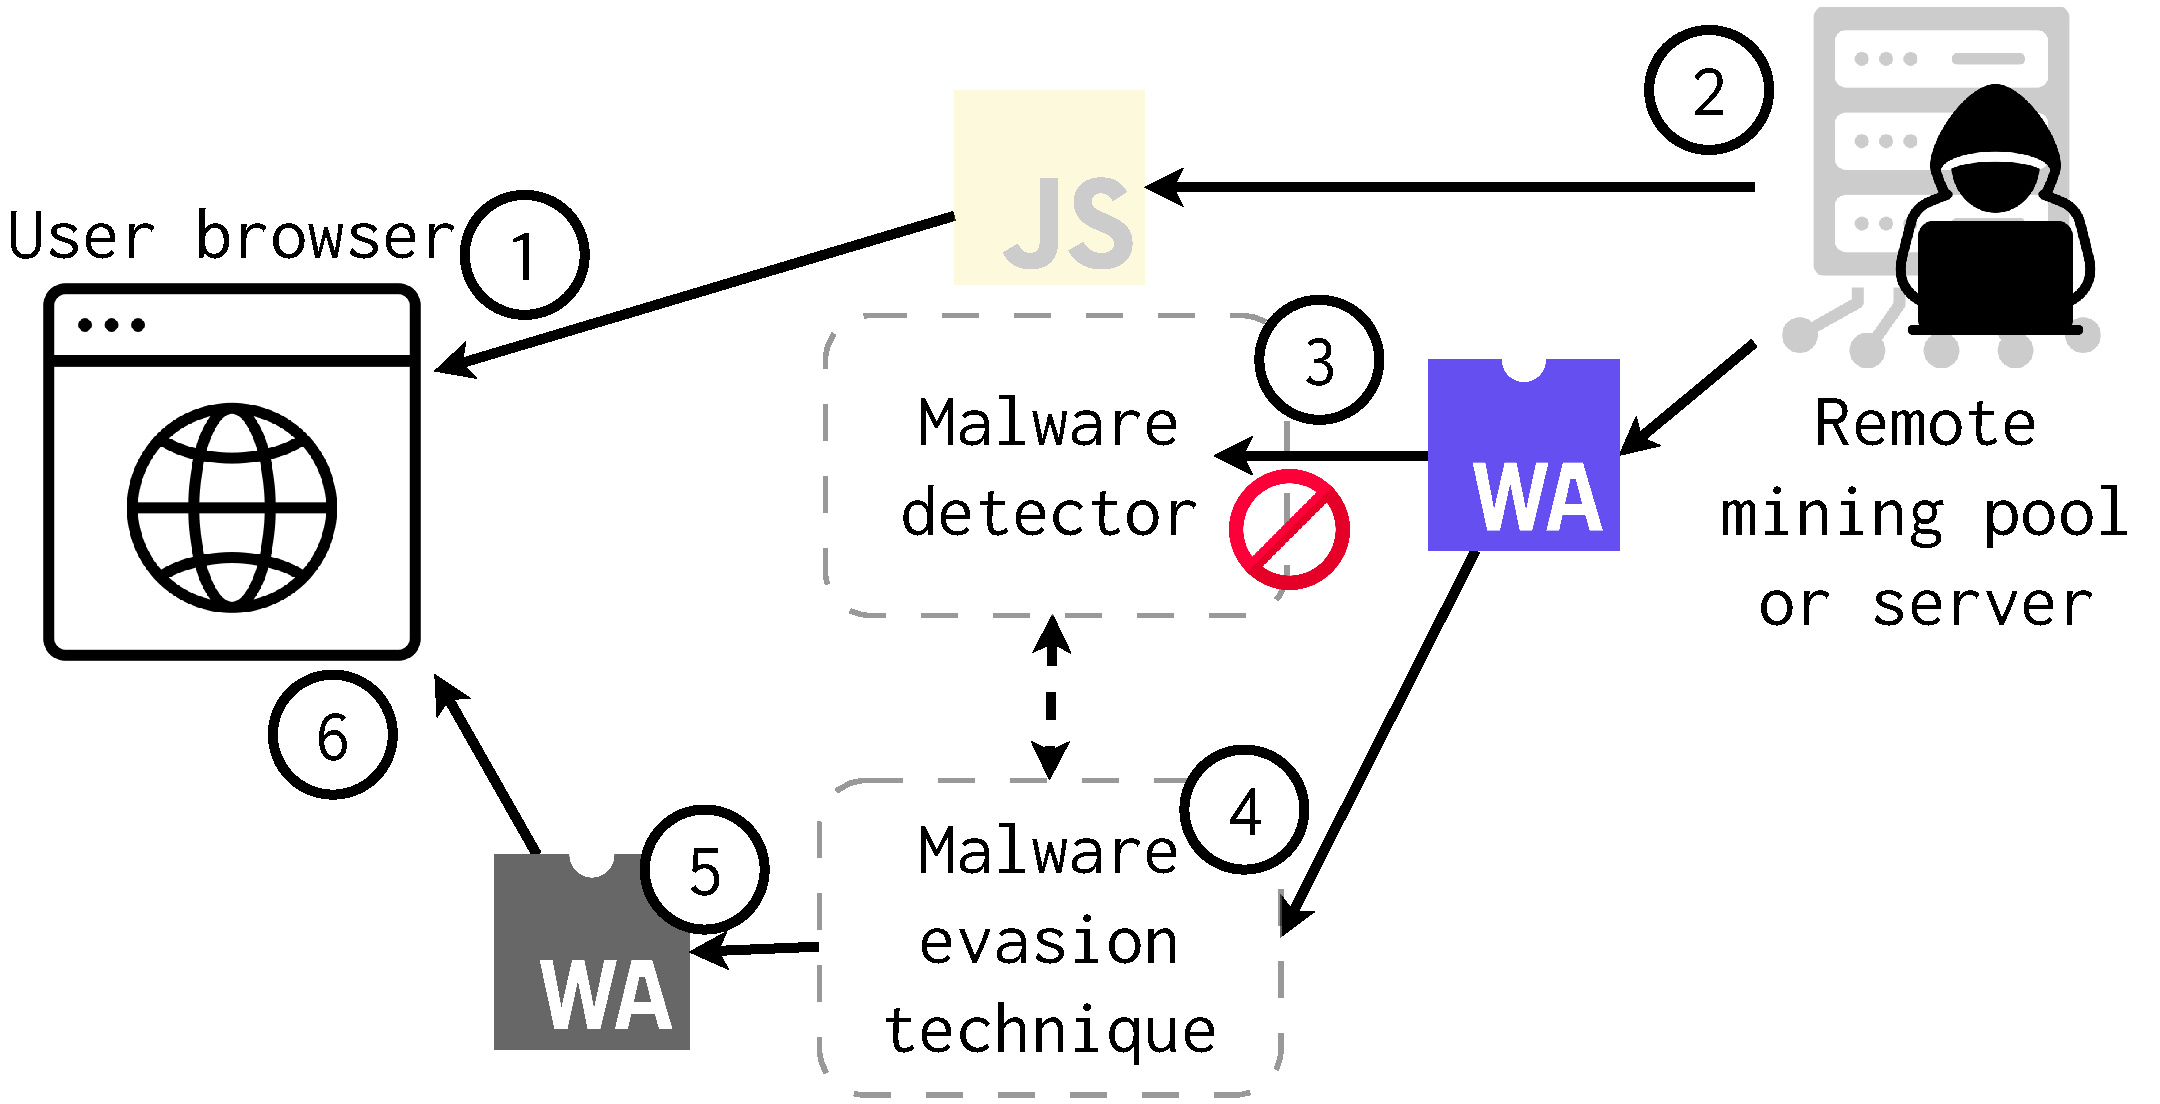
\includegraphics[width=0.8\linewidth]{figures/threat_model.pdf}
    \caption{Taken from \cite{EVASION}}
    \label{fig:threat_model}
\end{figure}

Test and evade the resilience of \Wasm malware detectors mentioned in \autoref{background:wasm:ecosystems}.


\msubsection{Approach}

%\lipsum[1]

\todo{We use wasm-mutate}
\todo{How do we use it?}
\todo{Controlled and uncontrolled diversification.}

%\lipsum[1]

%\lipsum[1]

\msubsection{Results}


\begin{tcolorbox}[title=Contribution paper,boxrule=1pt,arc=.2em,boxsep=1.0mm]
    The case discussed in this section is fully detailed in Cabrera-Arteaga \etal "WebAssembly Diversification for Malware Evasion"
    \emph{at Computers \& Security, 2023}
    \url{https://www.sciencedirect.com/science/article/pii/S0167404823002067}. 
\end{tcolorbox}
